\documentclass[runningheads]{llncs}

% ---- Encoding / Fonts ----
\usepackage[T1]{fontenc}

% ---- Figures / Tables ----
\usepackage{graphicx}
\usepackage{float}     % for [H] if needed
\usepackage{placeins}

% Subfigures (kept to preserve original \subfloat usage)
\usepackage{subfig}

% ---- Math ----
\usepackage{amsmath,amssymb}

% ---- Text / URLs ----
\usepackage{textcomp}
\usepackage{xcolor}
\usepackage{url}
\usepackage[hidelinks]{hyperref}

% Slightly tighter float placement (does not change margins/line spacing)
\renewcommand{\topfraction}{0.90}
\renewcommand{\bottomfraction}{0.90}
\renewcommand{\textfraction}{0.08}
\renewcommand{\floatpagefraction}{0.85}

\begin{document}

\title{Thermal Risk Monitoring in Electric Vehicle Batteries Using External Sensors and Machine Learning Algorithms}
\titlerunning{Thermal Risk Monitoring in EV Batteries}

% ---- BLIND REVIEW: no author identification ----
\author{Anonymous Author(s)}
\authorrunning{Anonymous Author(s)}
\institute{Anonymous Institute(s)}

\maketitle

\begin{abstract}
Thermal safety remains a critical challenge for electric vehicles, as abnormal temperature evolution in lithium ion batteries may lead to severe degradation or catastrophic failure. Conventional battery thermal monitoring is primarily performed by the Battery Management System, which relies on internal sensors, fixed thresholds, and proprietary data access. These characteristics limit adaptability to real world operating conditions and restrict deployment in retrofitted or third party scenarios. This paper presents a machine learning-based approach for battery thermal monitoring and early thermal risk awareness using exclusively external, non-intrusive temperature sensing. A low-cost sensing architecture based on an ESP32 microcontroller was developed to collect battery surface temperature, ambient temperature, and operational data during real-world riding experiments with an electric motorcycle. The collected telemetry was transmitted via a mobile gateway and processed in a backend infrastructure for temporal data analysis. Battery thermal behavior was modeled as a supervised regression problem with temporal dependence, and multiple machine learning algorithms, including K Nearest Neighbors, Decision Trees, Random Forest, Gradient Boosting, and Multilayer Perceptron, were evaluated. Results demonstrate that supervised learning models incorporating engineered temporal features can accurately capture battery surface temperature evolution, despite minor data losses and measurement noise. The findings indicate that external surface temperature measurements combined with temporally informed regression models can provide meaningful early thermal trend awareness without reliance on internal Battery Management System signals. This approach offers a practical, deployable, and non intrusive complementary safety layer for real world electric vehicle battery monitoring.

\keywords{battery thermal monitoring \and machine learning \and electric motorcycles \and real-world experiments}
\end{abstract}

\section{Introduction}
\label{sec:intro}

The thermal safety of electric vehicles (EVs) represents one of the most critical challenges currently faced by the automotive industry, as phenomena such as thermal runaway can lead to uncontrollable fires, severe material damage, and significant risks to human life~\cite{feng2018thermal,yang20196077,togun2025comprehensive}. Battery thermal monitoring is traditionally performed through the Battery Management System (BMS), which relies on internal sensors to supervise cell and module temperatures and to enforce operational safety limits~\cite{togun2025comprehensive,yang20196077}. However, these systems commonly depend on fixed thresholds or lookup tables derived from laboratory-based testing, which constrains their adaptability to the dynamic conditions of real-world operation and to the progressive aging of battery cells~\cite{yang20196077,li2023thermal,li2021datadriven}.

In addition, onboard BMS microcontrollers are subject to strict computational and memory constraints, limiting the deployment of advanced artificial intelligence algorithms directly at the vehicle level. In many practical scenarios, access to internal vehicle data through the Controller Area Network (CAN) bus is partial, noisy, or entirely unavailable, particularly in commercial or proprietary vehicle platforms. This lack of transparency undermines the reliability and generalizability of approaches that rely exclusively on internal signals such as voltage, current, state of charge (SOC), and internal temperature measurements~\cite{li2023thermal,li2021datadriven}.

Within this context, a notable gap can be observed in the literature regarding the use of external, non-intrusive sensors for battery thermal monitoring. The installation of internal sensors is often complex, costly, and difficult to retrofit in vehicles already in operation, whereas external clip-on temperature sensors offer a low-cost, flexible, and architecture-independent alternative~\cite{yang20196077,togun2025comprehensive,li2023thermal}. Nevertheless, data-driven approaches based on external sensing introduce additional challenges, including intermittent signal loss, asynchronous data transmission, and the influence of environmental conditions, all of which may degrade the accuracy of real-time thermal diagnostics~\cite{li2021datadriven,li2023thermal}.

In light of these limitations, this work proposes a machine learning--based approach for battery thermal monitoring and short-horizon temperature prediction that relies exclusively on temperature data collected by external, non-intrusive hardware. The proposed solution operates as an additional thermal monitoring layer, independent of the vehicle's internal parameters, and is designed to remain robust under conditions characterized by incomplete, noisy, or irregularly sampled data. By decoupling thermal risk assessment from proprietary BMS data, the proposed approach aims to improve the practicality and deployability of early thermal risk detection in real-world electric vehicle applications.

The main contributions of this work are as follows: 
(i) the design of a low-cost external sensing architecture for battery thermal monitoring in electric vehicles, based exclusively on non-intrusive sensors; 
(ii) the formulation of battery thermal trend monitoring as a supervised regression problem with explicit temporal context under real-world telemetry imperfections; 
(iii) an empirical comparison of multiple machine learning models for short-horizon battery surface temperature prediction; and 
(iv) an experimental demonstration that meaningful early thermal trend awareness can be achieved without access to proprietary BMS signals.

The remainder of this paper is organized as follows. Section~\ref{sec:related} reviews the related literature. Section~\ref{sec:metho} describes the proposed architecture and methodology. Section~\ref{sec:results} presents the experimental results. Finally, Section~\ref{sec:discussion} discusses the main findings, limitations, and future research directions.

\section{Related Work}
\label{sec:related}

\subsection{Battery Thermal Monitoring}
Battery thermal monitoring is commonly implemented within the Battery Management System (BMS) using internal sensors and internal vehicle data interfaces supervision~\cite{togun2025comprehensive,yang20196077}. Production systems often rely on fixed or semi-adaptive thresholds calibrated in laboratory conditions, which limits generalization to varying ambient conditions, heterogeneous vehicle platforms, and cell aging effects~\cite{togun2025comprehensive,yang20196077}.

\subsection{Anomaly Detection in EV Batteries}
Model-based methods use electrochemical and thermal models to detect deviations, but require accurate parameterization and can be sensitive to modeling errors~\cite{togun2025comprehensive,yang20196077}. Data-driven approaches using machine learning (e.g., random forests, neural networks) have been applied to identify abnormal behavior, typically assuming internal BMS measurements such as voltage, current, SOC, and internal temperature~\cite{li2023thermal,li2021datadriven}. Practical deployment is challenged by proprietary access, embedded resource constraints, and real-world data issues (missing samples, noise, intermittent connectivity).

\subsection{Machine Learning with Temporal Features for Thermal Systems}
Predictive models are increasingly used to anticipate temperature evolution and enable early risk awareness. Classical statistical time series models (e.g., ARIMA) rely on assumptions of linearity and stationarity that may degrade under nonlinear, non-stationary dynamics typical of EV operation~\cite{box2015timeseries}. Recent work explores machine learning and deep learning approaches (e.g., LSTM/GRU/TCN) for temperature prediction in thermal monitoring contexts~\cite{li2023thermal,kirchgaessner2021motor}, often framing the task as supervised learning with sequential inputs. However, many studies assume continuous high-quality internal sensing streams, which is not always available in real-world or retrofit scenarios.

\subsection{Research Gap Summary}
Overall, existing methods largely depend on internal BMS data channels and embedded sensing, limiting deployability across proprietary fleets. There remains a gap in approaches that (i) rely exclusively on external, non-intrusive temperature sensing, (ii) are robust to real-world telemetry imperfections, and (iii) formulate temperature prediction as supervised regression with explicit temporal context to provide early thermal trend awareness under real operating conditions.

\section{System Architecture and Methodology}
\label{sec:metho}

\subsection{Data Collection Architecture}

The data collection system followed a hybrid architecture integrating embedded sensing, a mobile gateway, and a backend infrastructure for storage and analysis, as illustrated in Fig.~\ref{fig:arch-datalogger}. The embedded unit was built around an ESP32 microcontroller, selected due to its low cost and native Bluetooth Low Energy (BLE) support, enabling continuous telemetry streaming in mobile environments.

The sensing layer comprised external DS18B20 sensors used to measure battery casing surface temperature, motor surface temperature, and ambient temperature. In addition, an MPU-6050 triaxial accelerometer captured vibration and acceleration patterns to characterize the vehicle operating regime.

Communication between the ESP32 and the gateway was performed via Bluetooth Low Energy. A mobile device acted as a data concentrator, receiving telemetry from the embedded unit and enriching the dataset with geolocation and instantaneous speed obtained from GPS. The consolidated data were then transmitted to a backend server and persisted in a MongoDB non-relational database to support temporal data management and subsequent analytical processing. An overview of the complete sensing and data acquisition architecture is presented in Fig.~\ref{fig:arch-datalogger}.

\begin{figure}[t]
\centering
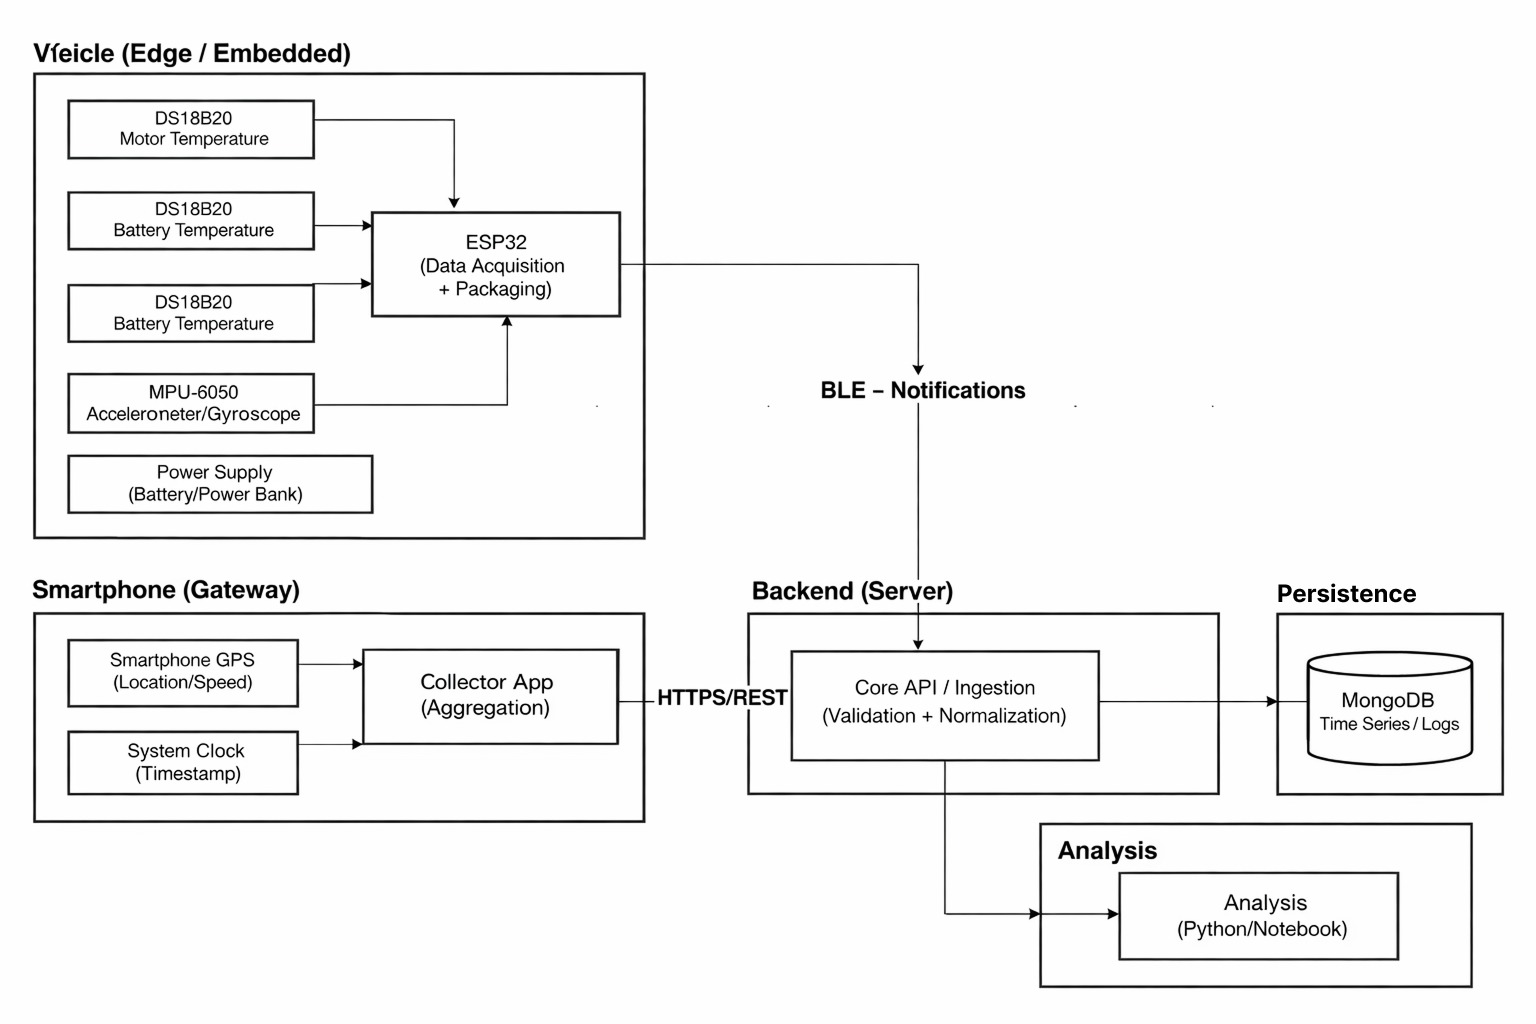
\includegraphics[width=0.9\textwidth]{img/arch-datalogger.png}
\caption{Architecture of the ESP32-based datalogger and data acquisition system used in this work.}
\label{fig:arch-datalogger}
\end{figure}

\subsection{Machine Learning Models for Temperature Prediction}
Thermal analysis was formulated as a supervised regression problem with temporal dependence to predict near-future battery surface temperature from historical external measurements and operational variables. Instead of employing classical statistical time series models, the approach relies on tabular machine learning algorithms trained on engineered features that encode temporal context (e.g., elapsed time and recent measurements). Unlike classical stochastic time series models, the adopted approach treats temperature evolution as a supervised regression task with engineered temporal descriptors rather than as a purely autoregressive stochastic process.

The evaluated models cover complementary bias--variance and interpretability trade-offs: KNN (local similarity), Decision Trees (interpretable baseline), Random Forest and Gradient Boosting (robust ensembles), and Multilayer Perceptron (nonlinear function approximation). This selection enables comparison across distance-based, tree-based, ensemble, and neural approaches under the same real-world telemetry constraints. This choice is also aligned with empirical evidence that tree-based ensembles often outperform deep models on typical tabular datasets~\cite{grinsztajn2022tabular,shwartz2021tabular,kishore2024temperature}.

\subsection{Experimental Data Collection Protocol}

Experiments were conducted using an electric motorcycle instrumented with the sensing system described in the previous section and connected to a smartphone for GPS-based acquisition. Three external temperature sensors monitored ambient temperature, motor surface temperature, and battery casing surface temperature. Data were collected during real-world rides along predefined urban routes. Each run lasted approximately ten minutes, allowing the capture of gradual thermal evolution under realistic operating conditions.

To induce operational variability, multiple riding modes were used across runs (Eco, Normal, Turbo), producing distinct power delivery profiles and thermal responses. Routes were repeated to ensure comparability and reproducibility of the measurements. GPS trajectories recorded during the rides were used to reconstruct route maps for each operating mode. An overview of the instrumented platform is presented in Fig.~\ref{fig:arch-datalogger}, while the reconstructed routes corresponding to the eco, normal, and turbo riding modes are shown in Fig.~\ref{fig:routes-by-mode}.

\FloatBarrier

\begin{figure}[!hbt]
\centering
\subfloat[Economic mode route]{%
  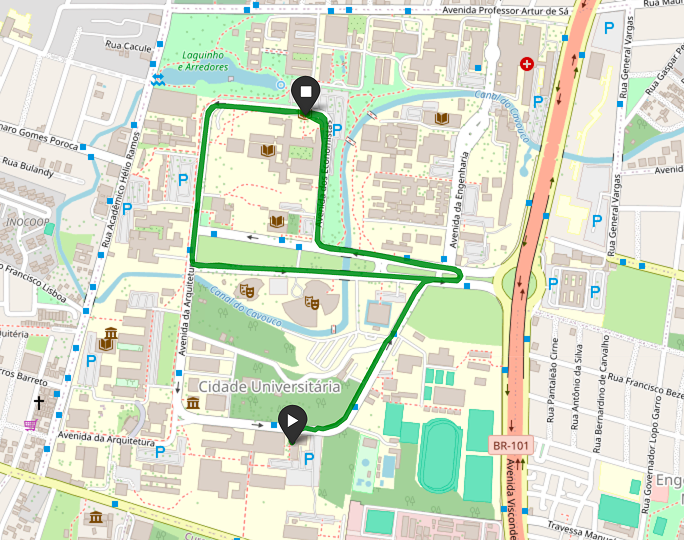
\includegraphics[width=0.31\textwidth]{img/map-eco.png}%
  \label{fig:map-eco}%
}
\hfill
\subfloat[Normal mode route]{%
  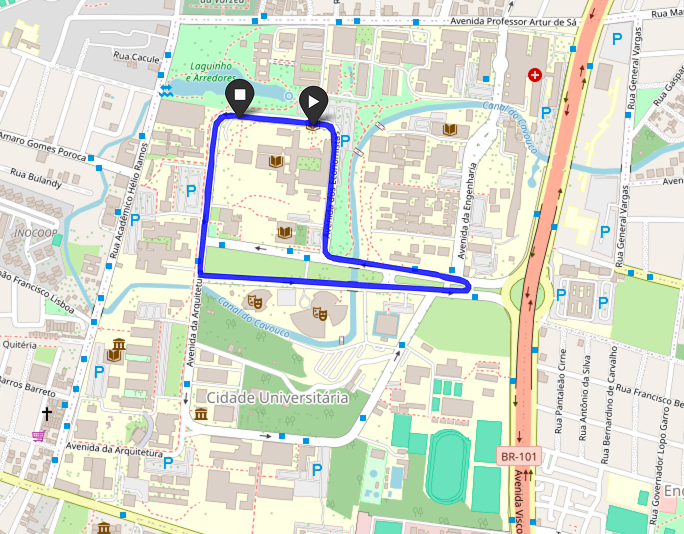
\includegraphics[width=0.31\textwidth]{img/map-nor.png}%
  \label{fig:map-nor}%
}
\hfill
\subfloat[Turbo mode route]{%
  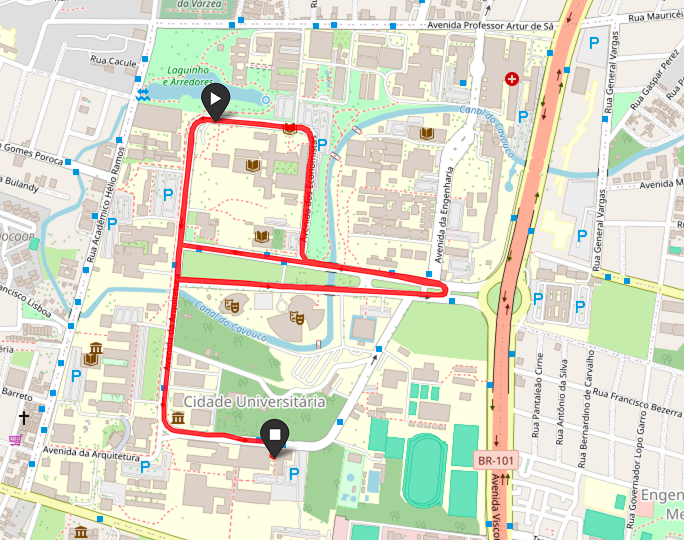
\includegraphics[width=0.31\textwidth]{img/map-tur.png}%
  \label{fig:map-tur}%
}
\caption{Reconstructed routes recorded during the experiments for the three vehicle operating modes: economic, normal, and turbo.}
\label{fig:routes-by-mode}
\end{figure}

\subsection{Data Preprocessing}

Telemetry exports were consolidated into a structured dataset containing timestamps, GPS coordinates, vehicle speed, accelerometer readings, and temperature measurements. Raw telemetry occasionally contained anomalous spikes caused by communication interruptions and sensor transmission artifacts. These implausible samples were removed during preprocessing to ensure temporal consistency and reliable downstream analysis. Figure~\ref{fig:preprocessing} illustrates an example of the raw temperature signals, in which occasional communication artifacts and implausible spikes can be observed prior to the cleaning stage.

Driving mode was encoded numerically, and elapsed time was computed relative to the start of each experimental run in order to capture temporal evolution effects. The resulting feature set included ambient temperature, vehicle speed, triaxial acceleration components, driving mode, and elapsed time, while battery casing surface temperature was used as the prediction target variable.

The dataset was divided into training and test subsets using an 80/20 split to evaluate generalization capability. Given the relatively small dataset size, the evaluation protocol is particularly important to avoid optimistic performance estimates and to ensure reliable validation of supervised learning models~\cite{vabalas2019validation,joseph2022split}.

\begin{figure}[!hbt]
\centering
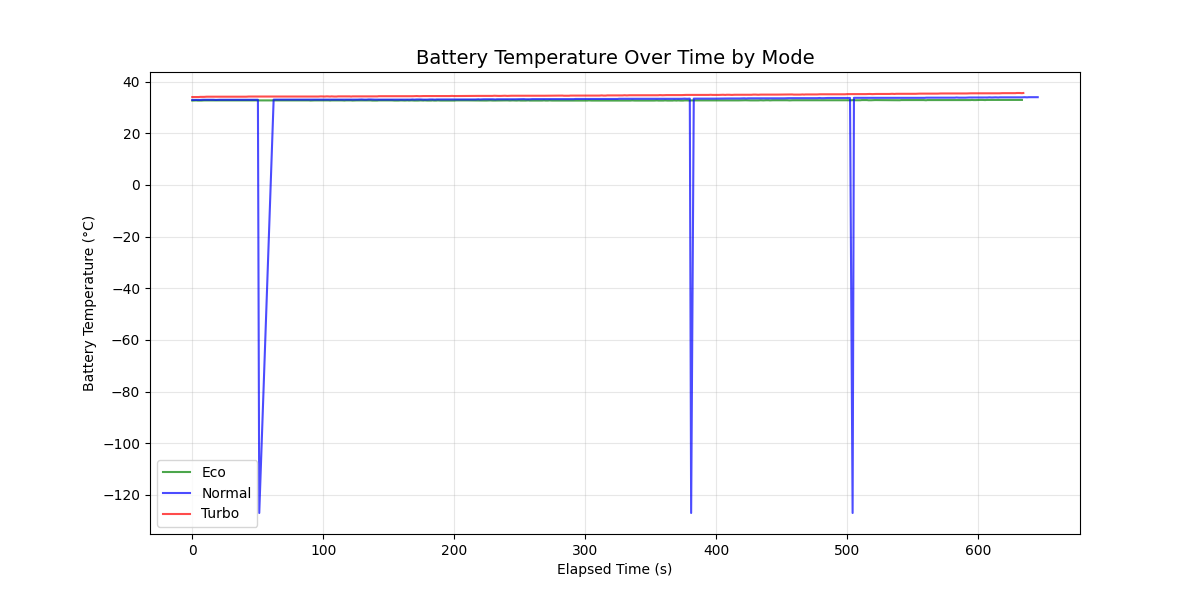
\includegraphics[width=0.75\textwidth]{img/battery_eda_evolucao_temp_escalar.png}
\caption{Example of raw battery temperature signals before preprocessing. Occasional spikes and discontinuities are associated with communication artifacts and sensor transmission failures.}
\label{fig:preprocessing}
\end{figure}

\subsection{Software Environment and Model Training}

The analysis workflow was implemented in Python using the pandas and NumPy libraries for data manipulation and preprocessing, while machine learning models were implemented using the Scikit-learn framework. Feature normalization was performed using \texttt{StandardScaler} to ensure comparable scales across variables.

Hyperparameter tuning was conducted using \texttt{RandomizedSearchCV} combined with cross-validation in order to explore the parameter space efficiently while limiting computational overhead. In addition to prediction accuracy, computational metrics including execution time, CPU utilization, and memory consumption were recorded during training in order to evaluate the performance--cost trade-off of the candidate models.

For each algorithm, the best estimator identified during hyperparameter search was retrained on the training subset and subsequently evaluated on the unseen test set to estimate real-world predictive performance.


\subsection{Regression-Based Thermal Risk Assessment}

Instead of directly performing fault classification, thermal risk awareness was derived from regression-based temperature prediction. Predicted temperature trajectories were compared against predefined safety thresholds derived from battery operational limits.

Sustained predicted growth trends or threshold exceedances were interpreted as early indicators of abnormal thermal behavior. This approach enables anticipatory monitoring without requiring labeled fault events or access to proprietary internal vehicle signals such as CAN bus data, which are often unavailable in commercial electric vehicles.


\section{Results}
\label{sec:results}


\subsection{Dataset Description}

After preprocessing and removal of invalid samples, the resulting dataset contained approximately one thousand synchronized records obtained from real-world riding experiments under three driving modes. Each record included battery surface temperature, ambient temperature, vehicle speed, triaxial acceleration components, elapsed time, and riding mode.

Descriptive statistics for the main variables of the treated dataset are summarized in Table~\ref{tab:desc-stats}.

\begin{table}[!ht]
\centering
\caption{Descriptive statistics for the treated dataset.}
\label{tab:desc-stats}
\scriptsize
\setlength{\tabcolsep}{4pt}
\begin{tabular}{lrrrrr}
\hline
Variable & Count & Mean & Std & Min & Max \\
\hline
Battery temperature (°C) & 1006 & 33.66 & 0.89 & 32.69 & 35.62 \\
Speed (m/s)              & 1006 & 9.03  & 4.27 & 0.00  & 19.05 \\
Acceleration X (mg)      & 1006 & 1096.6 & 233.0 & 167.0 & 2808.0 \\
Ambient temperature (°C) & 1006 & 31.88 & 0.49 & 30.44 & 33.12 \\
\hline
\end{tabular}
\end{table}

Minor data losses occurred due to transient communication or sensor interruptions, but preprocessing ensured temporal continuity of the dataset. The resulting data reflect realistic operational variability, including acceleration phases, cruising segments, stops, and speed fluctuations, providing a representative basis for thermal analysis and supervised regression modeling.


\subsection{Battery Thermal Behavior}

Across all experimental runs, battery surface temperature increased gradually and monotonically over time, reflecting the thermal inertia characteristic of lithium-ion battery systems. Heat generation during vehicle operation accumulates progressively, while heat dissipation to the environment occurs at a slower rate.

Higher power demand modes produced higher temperature levels and steeper temperature gradients, whereas lower demand modes exhibited more stable thermal behavior. After outlier filtering, no abrupt spikes or drops remained in the time series, indicating stable operation during the monitored sessions.

The temporal evolution and distribution of battery temperature across riding modes are illustrated in Fig.~\ref{fig:temp-analysis}, including the time-series profiles shown in Fig.~\ref{fig:temp-evolution} and the distribution summary presented in Fig.~\ref{fig:temp-boxplot}.

\begin{figure}[!hbt]
\centering
\subfloat[Temperature evolution]{%
  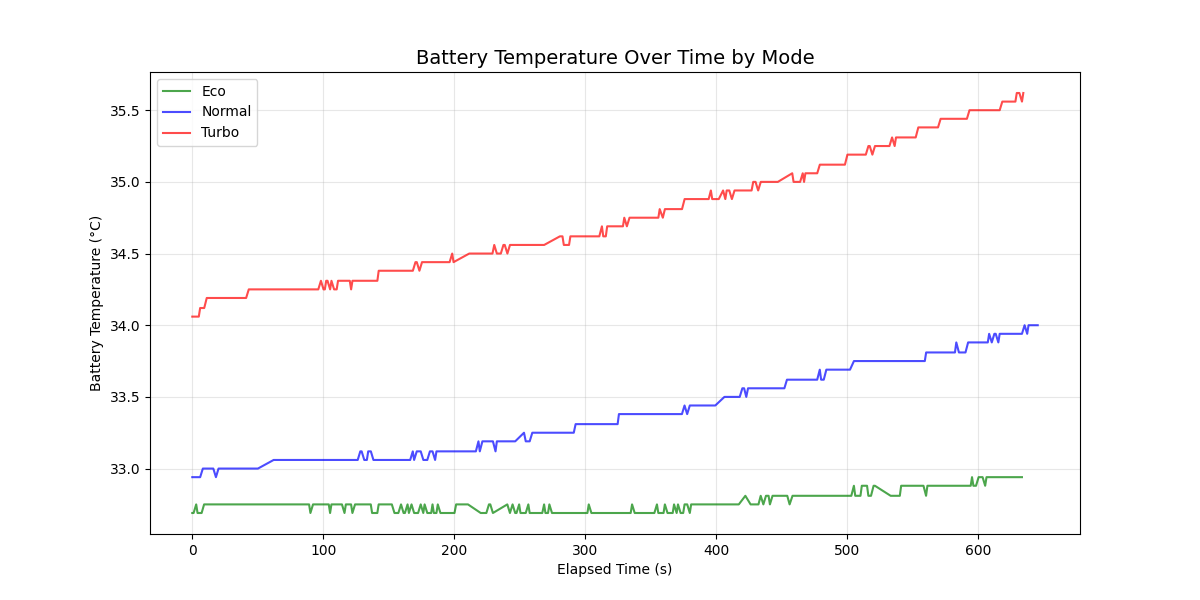
\includegraphics[width=0.48\textwidth]{img/battery_eda_evolucao_temp_tratados.png}
  \label{fig:temp-evolution}
}
\hfill
\subfloat[Temperature distribution]{%
  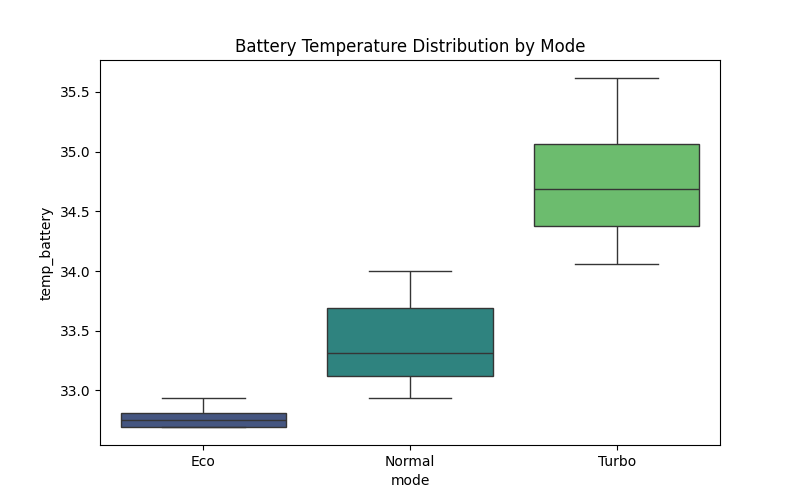
\includegraphics[width=0.48\textwidth]{img/battery_eda_boxplot_temp_tratados.png}
  \label{fig:temp-boxplot}
}
\caption{Battery temperature behavior across the three driving modes.}
\label{fig:temp-analysis}
\end{figure}


\subsection{Influence of Operating Conditions}

Driving mode exhibited a strong association with both temperature levels and temperature gradients. Vehicle speed and elapsed time also showed positive relationships with temperature evolution, reflecting cumulative energy consumption during operation.

Ambient temperature primarily influenced baseline temperature levels, while acceleration and vibration signals presented lower direct correlation with instantaneous battery temperature. Nevertheless, these signals contributed to characterizing the operational regime of the vehicle.

The multivariate relationships among the variables are summarized in Fig.~\ref{fig:analysis-and-performance}, which presents the correlation matrix in Fig.~\ref{fig:corr-matrix}.


\subsection{Observed Thermal Irregularities}

Exploratory inspection of the raw telemetry revealed occasional anomalous readings associated with communication artifacts rather than genuine thermal events. After preprocessing, the temporal profiles no longer exhibited spurious spikes or discontinuities.

No sustained overheating events occurred during the monitored sessions. Therefore, the evaluation focused on the ability of predictive models to capture temperature trends and anticipate potential abnormal thermal evolution rather than detecting actual failure events.


\subsection{Temperature Prediction Performance}

Machine learning models were evaluated for predicting battery surface temperature. Temporal features capturing thermal inertia significantly improved predictive accuracy compared to models relying only on instantaneous variables.

Tree-based ensemble methods and multilayer perceptrons provided strong alignment between predicted and observed temperature trajectories. Simpler models demonstrated higher sensitivity to noise and local variations in the data.

The high predictive accuracy observed for tree-based models can be partly explained by the smooth thermal dynamics and strong temporal autocorrelation present in the dataset.

Quantitative performance metrics and computational training costs are summarized in Table~\ref{tab:model-performance}. The correlation structure and comparative model performance overview are illustrated in Fig.~\ref{fig:analysis-and-performance}, including the correlation matrix (Fig.~\ref{fig:corr-matrix}) and the model comparison plot (Fig.~\ref{fig:model-performance}).

\begin{table}[!ht]
\centering
\caption{Prediction performance and training cost on the treated dataset.}
\label{tab:model-performance}
\scriptsize
\setlength{\tabcolsep}{4pt}
\begin{tabular}{lcccccc}
\hline
Model & $R^2$ & MAE (°C) & RMSE (°C) & Train time (s) & CPU (\%) & RAM (MB) \\
\hline
Random Forest     & 0.999 & 0.012 & 0.021 & 0.99 & 4.9  & 1735 \\
Decision Tree     & 0.999 & 0.012 & 0.025 & 0.10 & 9.9  & 1734 \\
Gradient Boosting & 0.998 & 0.024 & 0.035 & 0.76 & 10.8 & 1624 \\
MLP               & 0.990 & 0.065 & 0.086 & 2.20 & 2.2  & 1511 \\
KNN               & 0.975 & 0.073 & 0.137 & 0.11 & 9.3  & 1809 \\
\hline
\end{tabular}
\end{table}


\begin{figure}[!hbt]
\centering
\subfloat[Correlation matrix]{%
  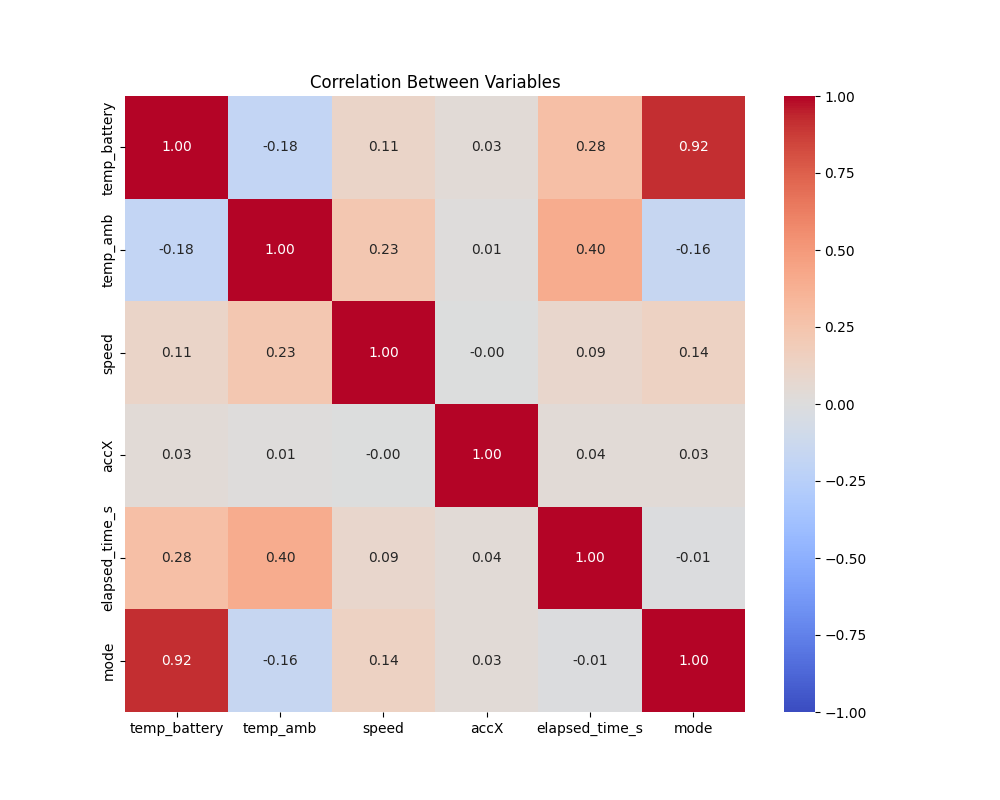
\includegraphics[width=0.48\textwidth]{img/battery_eda_correlacao_tratados.png}
  \label{fig:corr-matrix}
}
\hfill
\subfloat[Model comparison]{%
  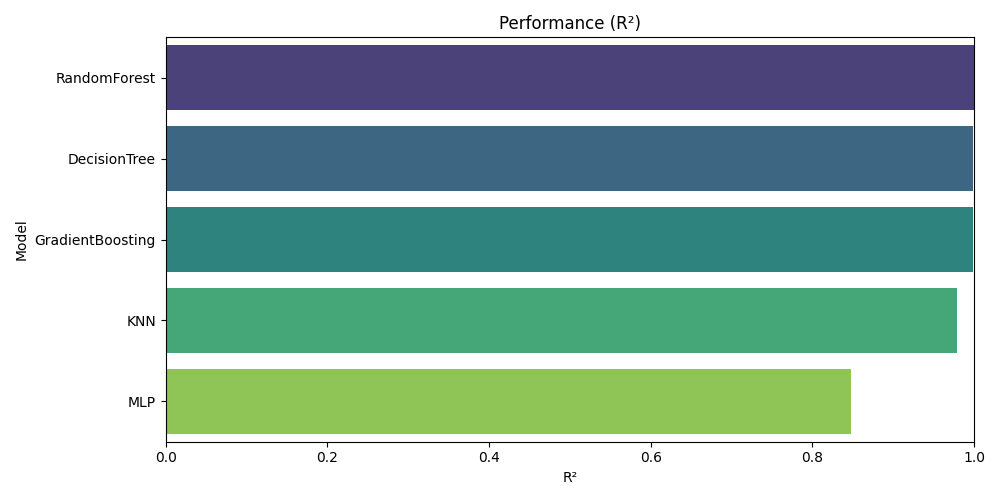
\includegraphics[width=0.48\textwidth]{img/battery_performance_modelos_tratados.png}
  \label{fig:model-performance}
}
\caption{Relationship analysis and predictive performance comparison across models.}
\label{fig:analysis-and-performance}
\end{figure}


\subsection{Early Overheating Detection}

Predicted temperature trajectories were compared against predefined safety thresholds representing acceptable battery operating conditions. Although no critical thermal events occurred during the experimental sessions, the supervised regression models successfully captured upward temperature trends ahead of time.

This demonstrates the feasibility of early thermal trend awareness using only external non-intrusive sensing combined with temporally informed machine learning models. Such an approach enables anomaly awareness without requiring labeled failure events or access to proprietary internal vehicle communication signals.

\section{Discussion and Conclusion}
\label{sec:discussion}
The observed gradual temperature dynamics are consistent with prior studies on battery thermal monitoring and anomaly detection that emphasize temperature evolution as a key safety indicator~\cite{feng2018thermal,togun2025comprehensive,yang20196077}. Unlike threshold-only strategies that react after conditions manifest, supervised regression with temporal context supports anticipatory awareness by projecting near-future temperature trajectories.

A central practical contribution is independence from internal BMS channels. Many existing methods rely on rich internal sensing and proprietary access, while this work demonstrates that external surface measurements combined with operational context can still provide meaningful trend awareness under real-world telemetry imperfections. This makes the approach potentially suitable as a complementary safety layer for retrofit or fleet monitoring scenarios where access to proprietary BMS channels is restricted.

Limitations remain: surface temperature is an indirect proxy for internal states and may lag fast fault escalation; sensor placement and environmental variability can influence readings; and the dataset reflects a single platform with no observed overheating events, restricting conclusions to trend awareness rather than validated failure prognosis. Future work requires broader vehicle diversity, longer-term data, and evaluation under more extreme thermal regimes.

\bibliographystyle{splncs04}
\bibliography{bibtex}

\end{document}